\documentclass[11pt,letterpaper]{article}

\addtolength{\oddsidemargin}{-.875in}
\addtolength{\evensidemargin}{-.875in}
\addtolength{\textwidth}{1.75in}

\addtolength{\topmargin}{-.875in}
\addtolength{\textheight}{1.75in}

\usepackage[utf8]{inputenc}
\usepackage{caption} % for table captions
\usepackage{amsmath} % for multi-line equations and piecewises
\DeclareMathOperator{\sign}{sign}
\usepackage{graphicx}
\usepackage{relsize}
\usepackage{xspace}
\usepackage{verbatim} % for block comments
\usepackage{subcaption} % for subfigures
\usepackage{enumitem} % for a) b) c) lists
\newcommand{\Cyclus}{\textsc{Cyclus}\xspace}%
\newcommand{\Cycamore}{\textsc{Cycamore}\xspace}%
\newcommand{\deploy}{\texttt{d3ploy}\xspace}%
\newcommand{\Deploy}{\texttt{D3ploy}\xspace}%
\usepackage{tabularx}
\usepackage{color}
\usepackage{multirow}
\usepackage{float}
\usepackage[acronym,toc]{glossaries}
\newacronym{ANL}{ANL}{Argonne National Laboratory}
\newacronym{B4C}{B4C}{boron carbide}
\newacronym{BC}{BC}{boundary condition}
\newacronym{BOC}{BOC}{beginning of equilibrium cycle}
\newacronym{BSD}{BSD}{Berkeley Software Distribution}
\newacronym{BWR}{BWR}{Boiling Water Reactor}
\newacronym{CAISO}{CAISO}{California ISO}
\newacronym{CEA}{CEA}{Commissariat a l'Energie Atomique}
\newacronym{CFD}{CFD}{computational fluid dynamics}
\newacronym{CO2}{CO$_2$}{carbon dioxide}
\newacronym{CR}{CR}{control rod}
\newacronym{CRP}{CRP}{Coordinated Research Project}
\newacronym{CZP}{CZP}{Cold Zero Power}
\newacronym{DCC}{DCC}{depressurized conduction cool-down}
\newacronym{DOE}{DOE}{Department of Energy}
\newacronym[\glslongpluralkey={degrees of freedom}]{DoF}{DoF}{degree of freedom}
\newacronym{EOC}{EOEC}{end of equilibrium cycle}
\newacronym{FCEV}{FCEV}{Fuel Cell Electric Vehicle}
\newacronym{FDM}{FDM}{Finite Difference Method}
\newacronym{FEM}{FEM}{Finite Element Method}
\newacronym{FVM}{FVM}{Finite Volume Method}
\newacronym{FSV}{FSV}{Fort St. Vrain}
\newacronym[\glslongpluralkey={greenhouse gases}]{GHG}{GHG}{greenhouse gas}
\newacronym{GRS}{GRS}{Gesellschaft für Anlagen und Reaktorsicherheit}
\newacronym{H2}{H$_2$}{hydrogen}
\newacronym{He}{He}{helium}
\newacronym{HFP}{HFP}{Hot Full Power}
\newacronym{HPCC}{HPCC}{high pressure conduction cool-down}
\newacronym{HTE}{HTE}{High-Temperature Electrolysis}
\newacronym{HTGR}{HTGR}{High-Temperature Gas-Cooled Reactor}
\newacronym{HTR}{HTR}{High Temperature Reactor}
\newacronym{HTTR}{HTTR}{High Temperature Test Reactor}
\newacronym{HZDR}{HZDR}{Helmholtz-Zentrum Dresden-Rossendorf}
\newacronym{IAEA}{IAEA}{International Atomic Energy Agency}
\newacronym{icap}{iCAP}{Illinois Climate Action Plan}
\newacronym{INL}{INL}{Idaho National Laboratory}
\newacronym{IPyC}{IPyC}{inner pyrolytic carbon}
\newacronym{JFNK}{JFNK}{Jacobian-Free Newton-Krylov}
\newacronym{KAERI}{KAERI}{Korea Atomic Energy Research Institute}
\newacronym{Keff}{K$_{eff}$}{multiplication factor}
\newacronym{LBP}{LBP}{Lumped Burnable Poison}
\newacronym{LGPL}{LGPL}{Lesser GNU Public License}
\newacronym{LOCA}{LOCA}{loss of coolant accident}
\newacronym{LPCC}{LPCC}{low pressure conduction cool-down}
\newacronym{LTE}{LTE}{Low-Temperature Electrolysis}
\newacronym{LWR}{LWR}{Light Water Reactor}
\newacronym{MC}{MC}{Monte Carlo}
\newacronym{MHTGR}{MHTGR}{Modular High-Temperature Gas-Cooled Reactor}
\newacronym{MOC}{MOC}{middle of equilibrium cycle}
\newacronym{MOOSE}{MOOSE}{Multi-physics Object-Oriented Simulation Environment}
\newacronym{MPI}{MPI}{Message Passing Interface}
\newacronym{MSR}{MSR}{Molten Salt Reactor}
\newacronym{MTD}{MTD}{Champaign-Urbana Mass Transit District}
\newacronym{NEA}{NEA}{Nuclear Energy Agency}
\newacronym{NEM}{NEM}{Nodal Expansion Method}
\newacronym{NGNP}{NGNP}{Next Generation Nuclear Power}
\newacronym{NRC}{NRC}{Nuclear Regulatory Commission}
\newacronym{NSC}{NSC}{Nuclear Science Committee}
\newacronym{OECD}{OECD}{Organisation for Economic Co-operation and Development}
\newacronym{OPyC}{OPyC}{outer pyrolytic carbon}
\newacronym{ORNL}{ORNL}{Oak Ridge National Laboratory}
\newacronym{OS}{OS}{Operator-Splitting}
\newacronym{PBMR}{PBMR}{Pebble Bed Modular Reactor}
\newacronym{PDE}{PDE}{Partial Differential Equation}
\newacronym{PMR}{PMR}{Prismatic Modular Reactor}
\newacronym{PV}{PV}{photovoltaics}
\newacronym{RSC}{RSC}{Reserve Shutdown Control}
\newacronym{RSD}{RSD}{Relative Standard Deviation}
\newacronym{SD}{SD}{Standard Deviation}
\newacronym{SI}{SI}{Sulfur-Iodine}
\newacronym{SiC}{SiC}{silicon carbide}
\newacronym{SMR}{SMR}{Small Modular Reactor}
\newacronym{SNU}{SNU}{Seoul National University}
\newacronym{SOEC}{SOEC}{Solid Oxide Electrolysis Cells}
\newacronym{TIP}{TIP}{transverse integration procedure}
\newacronym{TRISO}{TRISO}{Tristructural Isotropic}
\newacronym{UIUC}{UIUC}{University of Illinois at Urbana-Champaign}
\newacronym{UNIST}{UNIST}{Ulsan National Institute of Science and Technology}
\newacronym{UK}{UK}{United Kingdom}
\newacronym{UMICH}{UMICH}{University of Michigan}
\newacronym{US}{US}{United States}
\newacronym{VHTR}{VHTR}{Very High Temperature Gas Cooled Reactor}
%\newacronym{<++>}{<++>}{<++>}
%\newacronym{<++>}{<++>}{<++>}

\definecolor{bg}{rgb}{0.95,0.95,0.95}
\newcolumntype{b}{X}
\newcolumntype{f}{>{\hsize=.15\hsize}X}
\newcolumntype{s}{>{\hsize=.5\hsize}X}
\newcolumntype{m}{>{\hsize=.75\hsize}X}
\newcolumntype{r}{>{\hsize=1.1\hsize}X}
\usepackage{titling}
\usepackage[hang,flushmargin]{footmisc}
\renewcommand*\footnoterule{}
\usepackage{tikz}
\usepackage{array}
\usepackage{booktabs,mathptmx,siunitx}
\sisetup{input-symbols = {()},  % do not treat "(" and ")" in any special way
         group-digits  = false} % no grouping of digits

\usetikzlibrary{shapes.geometric,arrows}
\tikzstyle{process} = [rectangle, rounded corners,
minimum width=1cm, minimum height=1cm,text centered, draw=black,
fill=blue!30]
\tikzstyle{arrow} = [thick,->,>=stealth]

\graphicspath{}

\begin{document}

\section{\gls{PMR} neutronic solvers}

Nowadays there are several codes to solve the neutronics of \glspl{PMR}.
Most of them rely on the following methods: \gls{MC}, deterministic transport, and deterministic diffusion.
We focus our interest in the last method.
% Why? Deterministic diffusion solvers have lower computational requirements than other methods reference ??

The history of deterministic diffusion solvers begins in the late 1950s with the \gls{FDM} applied to the analysis of \glspl{LWR}.
In \gls{FDM}, mesh spacings are usually of the order of the diffusion length.
When solving large multi-dimensional problems, this limitation causes the mesh points to reach intractable numbers \cite{lewis_finite_1986}.
The computational expense of these calculations motivated the development of more computationally efficient techniques \cite{lawrence_progress_1985}.
Although there are substantial overlaps, the most common techniques fall into two broad categories: nodal methods and \gls{FEM}.

% --------------> LEFT HERE <----------------
% NODAL
From the 1970s, nodal methods proved to be a highly efficient and accurate technique in Cartesian geometries.
In 1981, a formulation based on \gls{NEM} first demonstrated the feasibility of nodal methods in hexagonal geometries \cite{duracz_nodal_1981}.

Nevertheless, this method would introduce non-physical singular terms that required the utilization of discontinuous polynomials.
This motivated the development of HEXNOD \cite{wagner_three-dimensional_1989} and HEXPEDITE \cite{fitzpatrick_hexpedite_1992}, more effective formulations introduced in the late 1980s and early 1990s.

HEXPEDITE's use still prevails in the analysis of \glspl{HTGR} \cite{ortensi_deterministic_2010-1}.
Some modern codes still use this technique.
DIF3D \cite{lawrence_dif3d_1983} and PARCS \cite{downar_parcs_2004} are examples of those codes.

% FEM
The \gls{FEM} is a well-established method in applied mathematics and engineering.
Most applications make \gls{FEM} preferable due to its flexibility in the treatment of curved or irregular geometries.
Also, the use of high order elements attains higher rates of convergence \cite{cavdar_finite_2004}.
The first prototype engineering application of \gls{FEM} was in the field structural engineering and dates back to 1956.
In the 1960s, \gls{FEM} became the most extensively used technique in almost every branch of engineering.
In 1981, \cite{lewis_finite_1981} described the first application of \gls{FEM} to the neutron diffusion theory.
Some examples of current \gls{FEM} diffusion solvers are Rattlesnake \cite{wang_rattlesnake_2019} and CAPP \cite{lee_development_2011}.

% More codes:
PHISICS (INL) % ref ?
Computes the time-dependent flux and power distribution in the core.
Is it FEM based?

% SPH treatment:
Others: PARCS (NRC), DIF3D-REBUS (ANL), APOLLO-CRONOS (AREVA)
\cite{gougar_htgr_2016}

\section{Thermo-Hydraulics}





\section{Multi-physics}
% HTGR benchmarks

Historically, linking a stand-alone neutronics solver to a thermal-hydraulics solver allowed for the simulation of an entire reactor.
For example, coupling PARCS, DIREKT, and THERMIX \cite{seker_analysis_2006} allowed for solving a \gls{PBMR}-400 Benchmark \cite{reitsma_oecdneansc_2006}.

RattleS$_n$ake \cite{wang_nonlinear_2013} has become the primary tool for solving the linearized Boltzmann neutron transport equation within \gls{MOOSE} \cite{strydom_inl_2013}.
RattleS$_n$ake counts with a variety of solvers available including low-order multigroup diffusion.
Pronghorn \cite{bingham_pronghorn_2012} \cite{novak_pronghorn_2018} is a \gls{FEM} porous media thermal-hydraulics simulation code built on the \gls{MOOSE} framework.

% More on Benchmarks
OECD PBMR400 Coupled Code Benchmark % ref ?
OECD/NEA MHTGR-350 Benchmark % ref ?
CRP on Uncertainty Analysis in HTRs % ref ?
\cite{gougar_htgr_2016}


\pagebreak
\bibliographystyle{plain}
\bibliography{bibliography}

\end{document}

	% \begin{figure}[htbp!]
	% 	\centering
	% 	\begin{subfigure}[t]{0.4\textwidth}
	% 		\centering
	% 		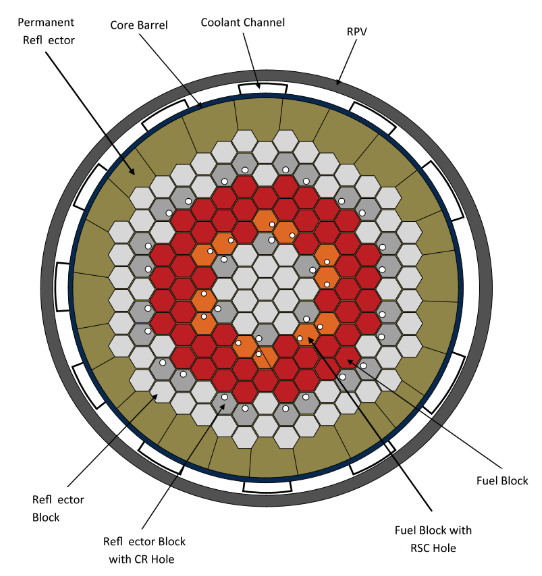
\includegraphics[width=\linewidth]{figures/radial-layout.png}
	% 		\caption{XY-plane.}
	% 	\end{subfigure}
	% 	\begin{subfigure}[t]{0.4\textwidth}
	% 		\centering
	% 		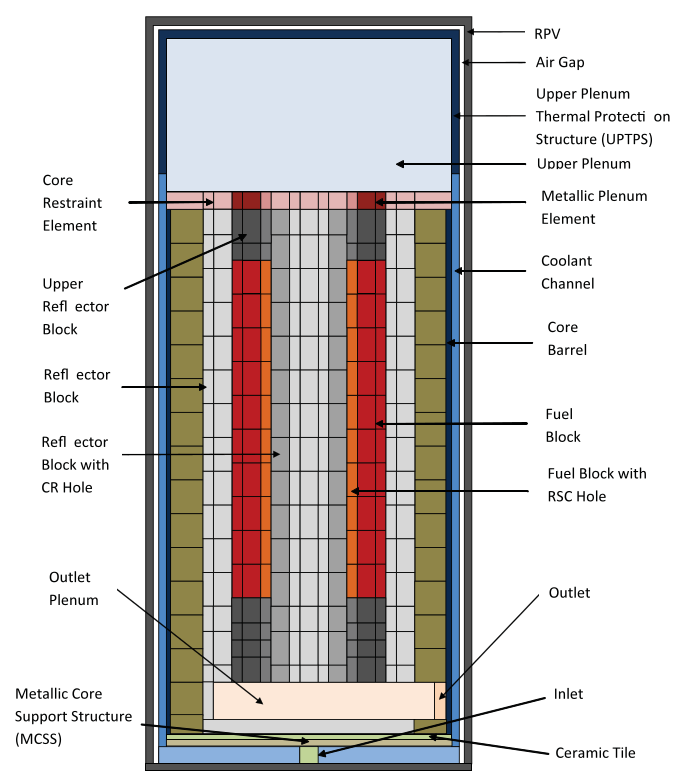
\includegraphics[width=\linewidth]{figures/axial-layout.png}
	% 		\caption{YZ-plane.}
	% 	\end{subfigure}
	% 	\hfill
	% 	\caption{MHTGR reactor layout.}
	% 	\label{fig:layout}
	% \end{figure}

	% \begin{figure}[htbp!]
	% 	\centering
	% 	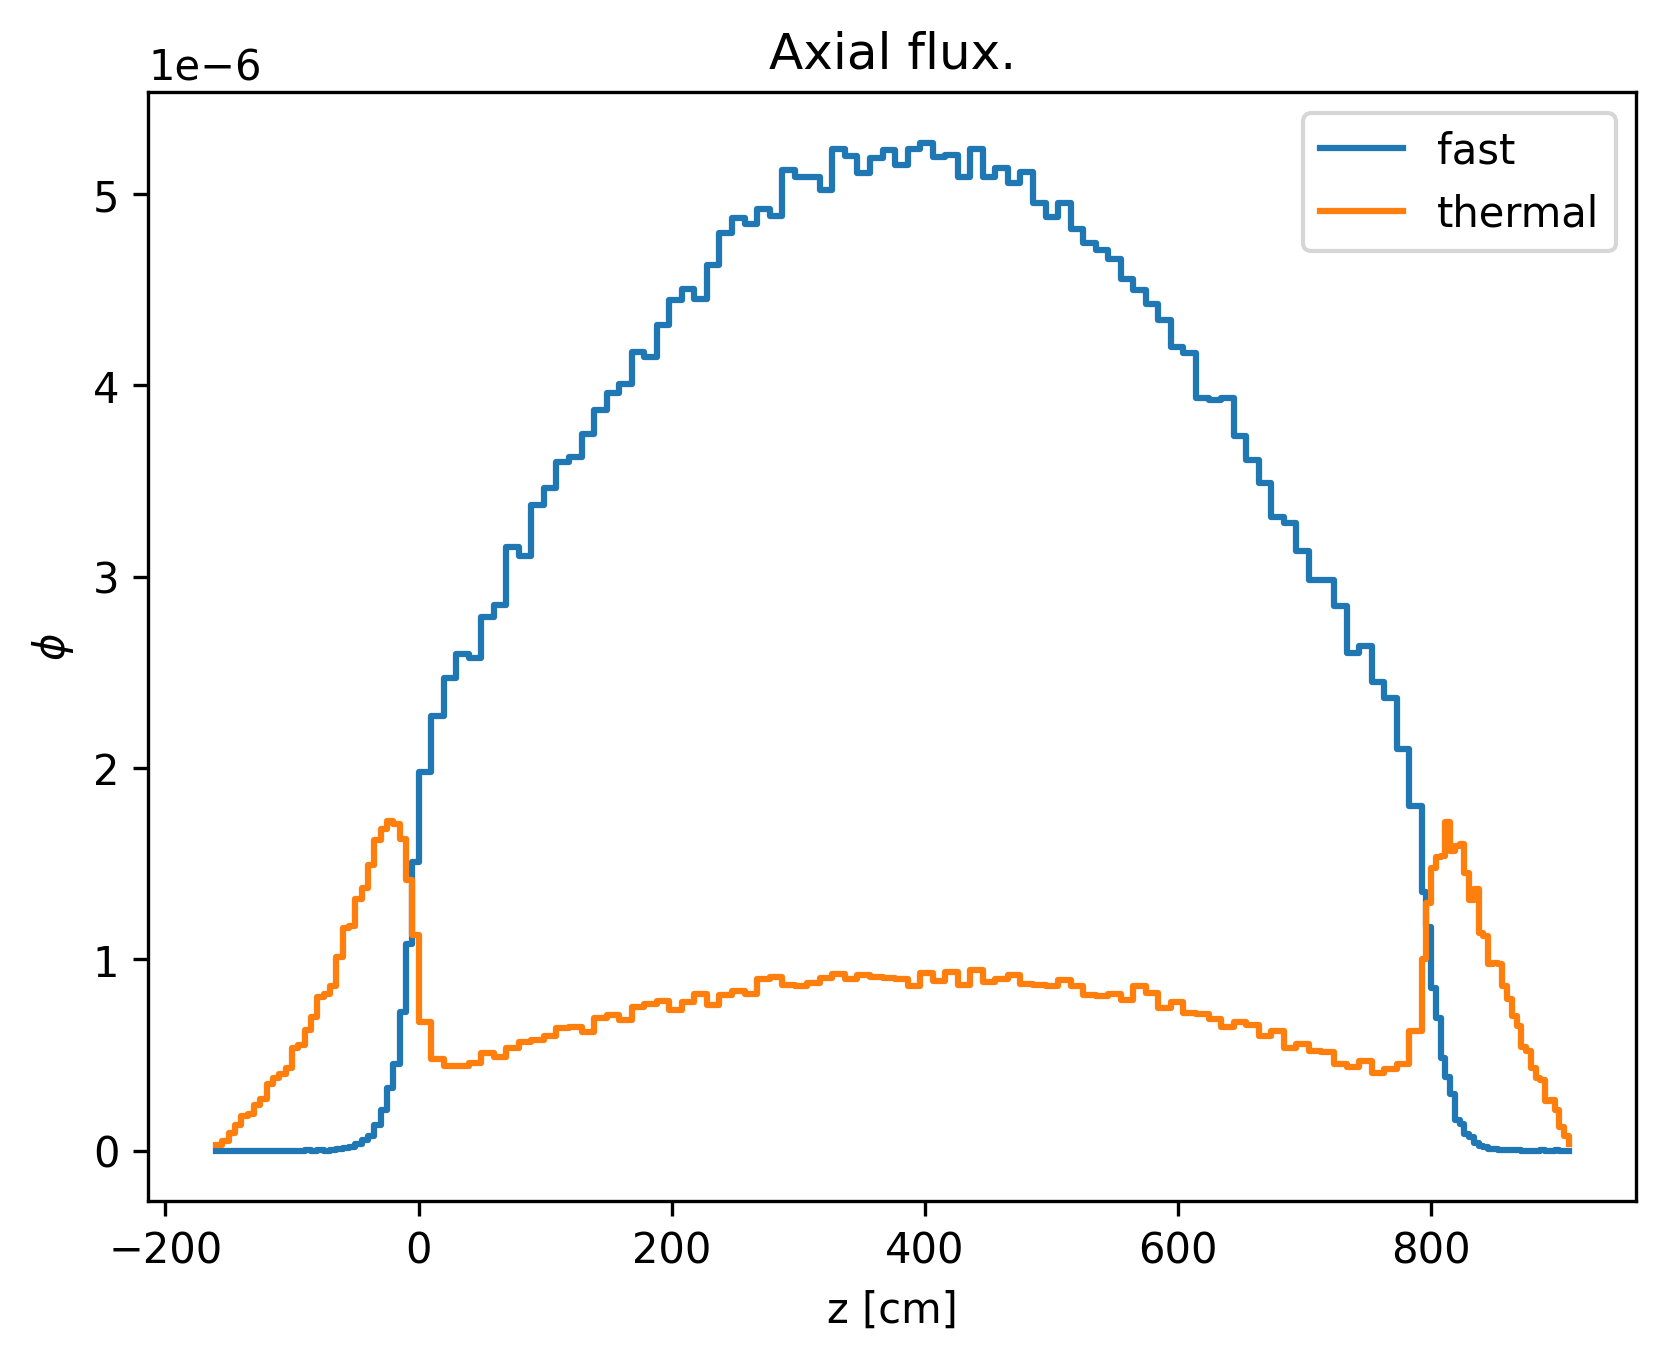
\includegraphics[width=0.6\linewidth]{figures/axial1.png}
	% 	\hfill
	% 	\caption{Neutron flux on the specified fuel channel.}
	% 	\label{fig:axial}
	% \end{figure}
